\documentclass{article}
\usepackage{graphicx}  % Pour inclure des images
\usepackage[french]{babel}  % Pour la langue française
\usepackage[T1]{fontenc}  % Encodage des caractères


\begin{document}

\title{Prototype }
\author{Tristan Petit, Nils Hubert, Toni Rey, \\ Majd El Sebeiti, Vianney Miquel}
\date{\today}

\maketitle

\section{Introduction}

Ce document regroupe un total de \textbf{n} captures d'écran accompagnées d'explications détaillées.

\section{Communication entre deux VM}

L'image ci-dessous illustre un ping entre la machine virtuelle de Toni et celle de Vianney, qui ne se trouvent pas sur le même hyperviseur.

\begin{figure}[h]
    \centering
    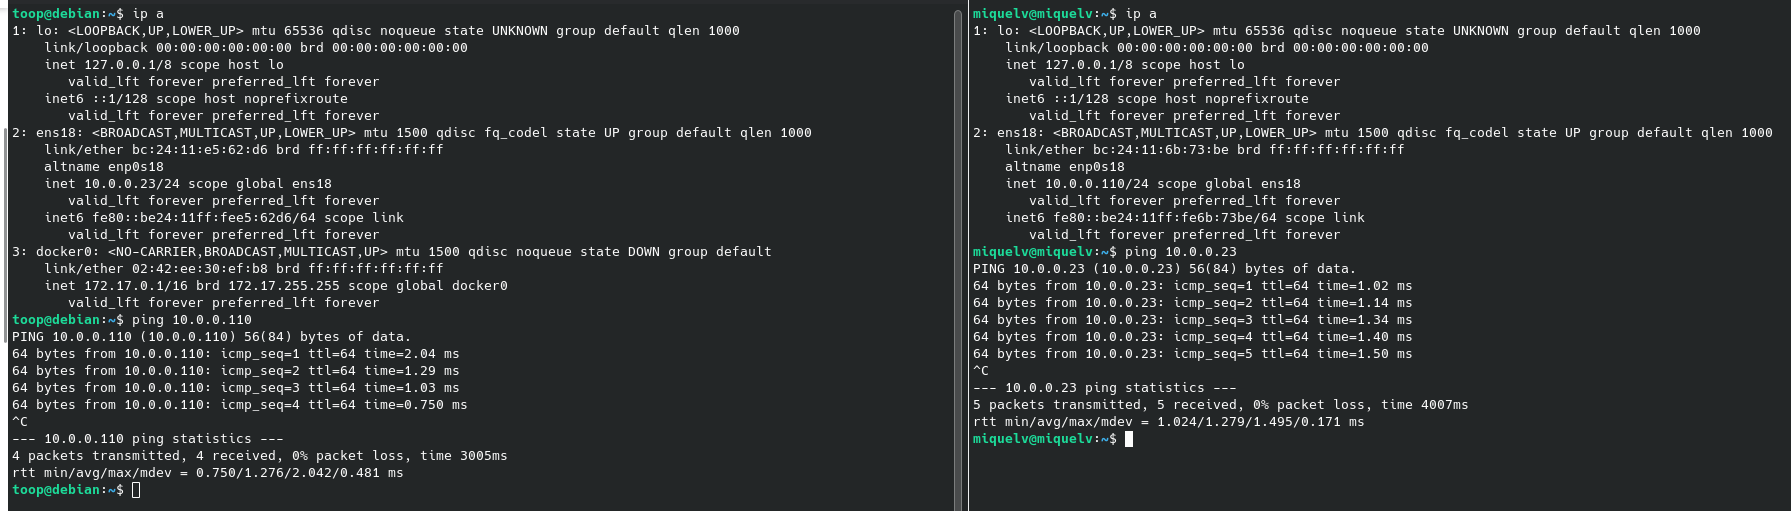
\includegraphics[width=0.8\textwidth]{Ping.png}
    \caption{Ping entre deux machines virtuelles sur des hyperviseurs distincts}
\end{figure}

\section{Accès à Internet}

L'image suivante montre un ping vers Google, prouvant ainsi que les machines ont bien accès à Internet.

\begin{figure}[h]
    \centering
    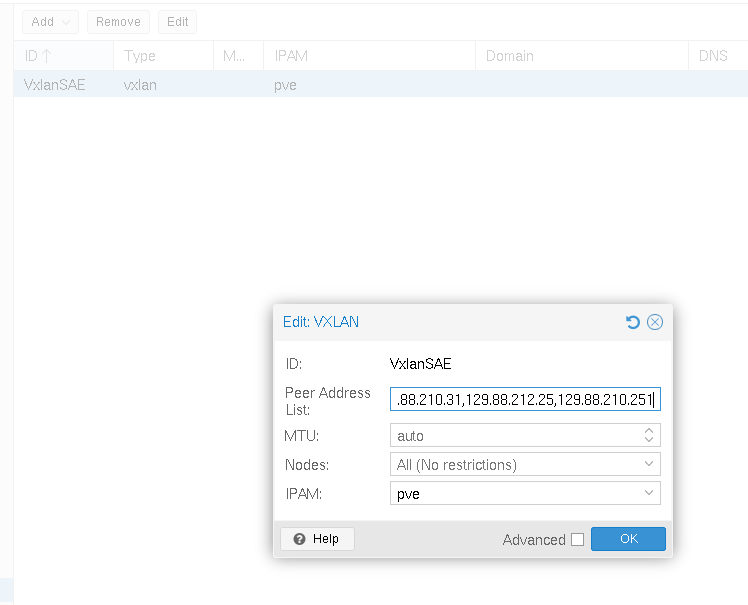
\includegraphics[width=0.8\textwidth]{VxLan.png}
    \caption{Test de connexion Internet avec un ping vers Google}
\end{figure}

\end{document}
